\documentclass[12pt]{article}

% Sets document language to English (some british conventions in
% hyphenation). Can also handle multilingual documents.
\usepackage[british]{babel}
\usepackage{csquotes}
\usepackage{pdflscape} 
\usepackage{geometry}
\usepackage{longtable}
\usepackage{gensymb}
\usepackage{listings}
\usepackage{caption}
\usepackage{subcaption}
\usepackage{tabularx}
\usepackage{listings}
\lstset{
  tabsize=2,
  breaklines=true,
  captionpos=b,
  extendedchars=true,
  numbers=left,
  basicstyle=\ttfamily,
  commentstyle=\color{red!70!black},
  keywordstyle=\color{green!70!black},
  numberstyle=\tiny\color{black!50},
  stringstyle=\ttfamily\color{blue!50!black},
  backgroundcolor=\color{yellow!10}
}

% Uses the newer biblatex (with biber as backend) for citations and
% references. Can deal with non-ascii letters in author names.
\usepackage{biblatex}
\addbibresource{references.bib}

% Provides more maths support and the theorem environments.
\usepackage{amsmath}
\usepackage{amsthm}
\theoremstyle{plain}
\newtheorem{theorem}{Theorem}
\newtheorem{lemma}[theorem]{Lemma}
\theoremstyle{definition}
\newtheorem{definition}[theorem]{Definition}

% Font handling here is intended for LuaTeX or XeTeX engine.
% Sets the font. In this case a font similar to Times.
\usepackage{fontspec}
\setmainfont{TeX Gyre Termes}
\setmonofont{Source Code Pro}[Scale=MatchLowercase]
% Unicode math fonts
\usepackage{unicode-math}
\setmathfont{texgyretermes-math.otf}

% Some generally useful packages:
% Provides \includegraphics to insert images.
\usepackage{graphicx}
% Provides \url to insert url links.
\usepackage{url}
% Provides colour support.
\usepackage{xcolor}
% Provides tables that are aesthetically more pleasing.
\usepackage{booktabs}
% Provides more configurable itemised and enumerated lists.
\usepackage{enumitem}
% Provides environment for defining vector graphics drawings.
\usepackage{tikz}
% Provides environment for code listings.
\usepackage{listings}
\lstset{
  tabsize=2,
  breaklines=true,
  captionpos=b,
  extendedchars=true,
  numbers=left,
  basicstyle=\ttfamily,
  commentstyle=\color{red!70!black},
  keywordstyle=\color{green!70!black},
  numberstyle=\tiny\color{black!50},
  stringstyle=\ttfamily\color{blue!50!black},
  backgroundcolor=\color{yellow!10}
}
% Provides hyperlinks in the pdf. Not suitable for printed documents,
% but fine here.
\usepackage[pdfborder={0 0 0},colorlinks=true,allcolors={blue!40!black}]{hyperref}

% Load the style file (title page and declarations) for the document.
\usepackage[]{swanseaTitleUG}

% Paragraphs are typeset with a small skip between them.
\usepackage[parfill]{parskip} 

% User supplied information that appears on title page. Do edit these!
\title{ Shoulder Surfing Detection}
\author{Katie Peacey}
\studentid{2214646}
\project{Shoulder Surfing Detector}

% Table of contents only lists 2 levels.
\setcounter{tocdepth}{2}

\begin{document}
\pagenumbering{roman}

\maketitle
\studentdeclarations

\begin{frontmatterparagraph}{Abstract}
Shoulder surfing is the act of visually observing someone’s private screen interactions without their consent and remains a significant privacy concern in public and semi-public spaces. From entering passwords at ATMs to composing confidential emails on laptops in cafes, users are increasingly vulnerable to visual eavesdropping. Past work on solutions such as physical privacy screens or behavioural adjustments often require users to alter their behaviour or purchase additional hardware, however these approaches frequently compromise usability, reduce screen visibility or demand constant user vigilance. This paper introduces a software-based shoulder surfing detection system developed using Python. The system uses real-time gaze tracking to identify the presence of unauthorised viewers and responds by sounding an alert and dimming the display to obscure sensitive content. The system has been designed  with the user experience in mind, so seeks to be non-intrusive and responsive to the user context indicating a strong potential for broader application across both mobile and desktop platforms.
\end{frontmatterparagraph}

% Build the table of contents page.
\tableofcontents

% These lists are optional, especially if they are empty.
\listoffigures
\listoftables
\clearpage

% Reset numeric page numbering from page 1
\pagenumbering{arabic}

\section{Introduction}
\label{sec:intro}

As mobile computing becomes more embedded in daily life, individuals are more likely to interact with laptops, tablets, and smartphones in public spaces such as cafes, libraries, offices, or public transport. This exposure increases security and privacy concerns including the risk of shoulder surfing, which is the act of observing someone else’s screen to gather privacy or sensitive information without their consent.

Shoulder surfing can occur both deliberately and inadvertently. In its deliberate form, an attack may position themselves behind or beside a victim to watch as they enter passwords, read sensitive emails, or access personal data. Inadvertent cases can involve passers-by or nearby users unintentionally glancing at a screen due to curiosity or proximity, still resulting in an invasion of privacy. Eiband et al. describes shoulder surfing as both a common and underestimated threat, particularly in environments where users are less aware of their surroundings \cite{eiband_understanding_2017}. Similarly, research by Aviv et al. demonstrates how observational attacks can be used to accurately extract PINs, swipe patterns, and alphanumeric passwords with minimal effort \cite{aviv_towards_2017}.

The risk associated with shoulder surfing is not limited to password theft as attackers can also capture financial details, health records, business correspondence or even biometric data by simply watching a screen. As these attacks often require no technical skill and can be carried out using the naked eye or a camera, their easy method of attack makes them especially concerning \cite{block_impact_2010}. In addition, modern device screens with high brightness and wide viewing angles inadvertently help attackers by making the screen contents visible from wider perspectives.

Given these risks, mitigating shoulder surfing has become an important factor within security. Past solutions, such as privacy screen protectors or alternative authentication solutions such as Passface \cite{liu_passface_2021} and Draw-a-Secret (DAS) \cite{nali_analyzing_2004}, have shown some success but often rely on hardware or suffer from poor long-term usability. These approaches can interrupt normal user behaviour or degrade the user experience allowing for an interest in a protection method that can integrate easily into users’ everyday interactions.

This paper introduces a gaze-based detection system as a productive solution to shoulder surfing. Implemented in Python, the system utilizes computer vision and gaze estimation techniques to monitor the presence of faces within a device’s camera view. When more than one face is detected and the user’s gaze is focused on the screen, the system triggers a subtle alert, such as screen dimming or an audio cue, to warn the user of a potential privacy threat.

The primary aim of this project is to develop a lightweight, software-only solution that identifies shoulder surfing attempts in real-time without interrupting the user’s workflow. To achieve this, the system is designed to be unobtrusive, user-friendly, and adaptable across various public or shared environments. The objectives include:

\begin{itemize}
  \item Implementing face detection and gaze tracking techniques suitable for real-time use.
  \item Designing a responsive user interface that allows users to customise detection sensitivity and feedback settings.
  \item Evaluating the system’s accuracy, usability, and effectiveness through controlled user studies.
  \item Iteratively refining the system based on user feedback and performance data.
\end{itemize}

These objectives create a focus of the practical usability of the system whilst ensuring it is reliable enough to detect any potential threats. his paper presents a review of related work, details the design and implementation of the system, and evaluates its performance and user experience through a structured study to offer a novel approach to mitigate shoulder surfing attacks.

\section{Related Work}
\label{sec:Related Work} 

Shoulder surfing is an increasingly prevalent issue. The occurrence of shoulder surfing is not limited to malicious attacks, it also includes unintentional glances and peeking out of interest. Research by Eiband et al. (2017) demonstrates that shoulder-surfing is commonplace, especially on public transportation and in communal environments. Their study suggests that users often lack awareness of being observed and generally underestimate the risk. Similarly, studies by Aviv et al. (2017) and De Luca et al. (2014) show how attackers can retrieve PINs and passwords through observational techniques, emphasising the urgency of practical mitigation strategies.

The earliest responses to shoulder surfing have been physical: privacy filters and screen covers (Lian et al. 2013). These accessories reduced the screen’s visibility angle to deter side glances from others. However, they also reduce usability for the primary user, especially in shared or collaborative settings. Something more about physical defences... 

Something about software-based defences. For example, Wiedenbeck et al. (2005) evaluated the DAS (Draw-a-secret) approach, while Tari et al. (2006) explored PIN-entry systems that reduce predictability. Though promising, these methods often compromise efficiency and are reflected by users for being cumbersome (Kroeze & Olivier, 2008).

Computer vision techniques have gained traction for dynamic user-aware defences. Brudy et al. (2014) introduced methods to detect onlookers in the context of public displays, while Khamis et al. (2016) explored gaze-based user interfaces that adapt to attention shifts. Real-time face detection, such as YOLO (You-Only-Look-Once)(Redmon et al. 2016), provides a fast and accurate way to identify multiple individuals in a frame. Insert YOLO facts here. This will be further discussed.

Gaze interaction has been increasingly used not only for input but also for context awareness and security. Holland and Komogortsev (2012) demonstrated that haze can be used for continuous authentication, while Kumar et al. (2007) showed gaze patterns can distinguish between users. Recent work by Liu et al. (2007) investigates how gaze cues can signal environmental risks without interrupting primary tasks. Such ambient strategies align closely with Weiser and Brown’s (1996) concept of calm technology interfaces that remain in the background until needed.

Something about UX. Research by Cranor and Garfinkel (2005) and more recent works by Nappa et al. (2019) confirm that users resist tools that are overly intrusive or complex. This proves that the most effective solutions are those that operate passively, offer user control and integrate smoothly into daily workflows.

Our system stands in the intersection of these lines of research. It bridges the high-performance detection with subtle, user-oriented alerts, guided by formative research in UX and informed by the limitations of past solutions.

\section{System Design}
\label{sec:system design}

\subsection{Overview of the system}
\label{sec:Overview of the system}

The proposed solution is a software-based approach that detects potential shoulder surfing by using gaze tracking. It was developed in Python with a focus of usability, responsiveness and adaptability within different environments. The solution aims to minimise user disruption by only providing feedback when a potential threat is detected.

The system uses a live video input combined with a gaze tracking algorithm to determine whether a user is being observed. The central idea is to detect multiple faces within the webcam view and compare this to the gaze direction to decide whether an unauthorised person is looking at the user’s screen. Once detected, the system triggers a response where the screen brightness is reduced, and an audio alert plays to notify the user discreetly. The user can remain in control of the system via a graphical interface with start/stop buttons and customizable settings.

\subsubsection{Human-Centred Design and UX Principles}

The system was designed following established Human-Computer Interaction (HCI) principles, with particular reference to Nielsen’s usability heuristics and Don Norman’s principles of design. Rather than overwhelming users with intrusive pop-ups or constant alerts, the system alights with Norman’s idea of making important system state visible and providing natural mappings between intentions and outcomes. We ensured that feedback is delivered through screen dimming and subtle sounds which allow for clear communication without demanding excessive attention.

The interface supports discoverability and feedback as per Norman’s principles by allowing adjustable settings that can be easily understood and controlled. The settings allow for the screen brightness when dimmed to be altered using a sliding bar and alert sounds can be toggled on and off. We have also ensured that the layout is simple by using minimal buttons, clear labels and consistent interaction patterns so that the user can easily use the system through recognition an have a minimal chance of making errors (Neiman, 2019).

\subsubsection{Privacy and Local Processing}

The system was built with privacy by design in mind, so all data processing occurs locally on the user’s device and no images or videos are saved, transmitted, or stored. This approach aligns with GDPR principles and reassures users that their data remains under their control. Since the webcam feed never leaves the device and is not stored in any form, the system supports high standards of personal data protection.

\subsection{Architecture}
\label{Architecture}
The software works by capturing live video input using the OpenCV library, which provides an efficient way to access real-time video streams. Rather than storing video feeds, frames are processing in real time to identify potential privacy threats.

For face detection, the system makes use of the dlib library’s Histogram of Oriented Gradients (HOG)-based face detector where detection speed and accuracy are computationally efficient to identify presence of more than one person. Upon detecting a face, the system applies dlib’s 68-point facial landmark model to identify specific points around the eyes needed for gaze estimation. 

Using the key eye landmarks, the system estimates gaze direction through geometric calculations where the relative position of the pupil within the eye socket and alignment with eye corners is used to infer whether the user is focused on the screen. Detection logic can then flag a potential shoulder surfing threat when multiple faces are present, and the user’s gaze is focused on the screen.

When a threat is detected, the system initiates feedback to the user by dimming the screen using the screen\textunderscore brightness\textunderscore control library and plays an alert sound to attract the user’s attention. The user interface has been built with customtkinter which provides an interactive control panel that includes start and stop buttons, a live video preview and a log of recent detection events for transparency and usability. 

In the initial prototype, YOLO (You Only Look Once) was used for person detection due to its high-speed object recognition, however in further development, this was replaced with dlib to enable integrated facial landmark tracking for gaze estimation. Justification for this is discussed further in the paper.

Figure~\ref{fig:architecture} demonstrates the flow of the system and how the architecture has been built in a modular way to allow for improvements and further research.

\begin{figure}[h!]
    \centering
    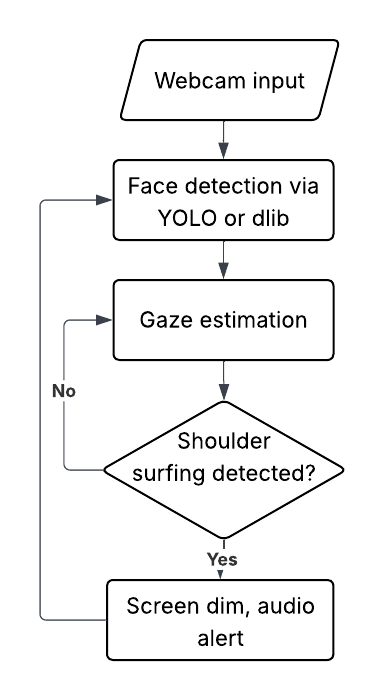
\includegraphics[width=0.3\linewidth]{img/architecture.png}
    \caption{Diagram to show the overall system architecture flow of the proposed solution.}
    \label{fig:architecture}
\end{figure}


\subsubsection{YOLO (You Only Look Once)}
During early development of this project, an object detection algorithm called YOLO \textcolor{red}{ref here} was identified as a suitable method for detecting the presence of onlookers.
YOLO (You Only Look Once) is an object detection algorithm produced in 2015 by Redmon et al. which uses bounding boxes to predict the probability of what each object is \cite{redmon_you_2016}. The algorithm has been trained using the ImageNet dataset \cite{noauthor_imagenet_nodate} and can detect from traffic lights to toilets. The YOLO model splits each image into a grid and produces bounding boxes for each cell, a class probability is listed, and a confidence score is calculated. The class probability is the likelihood that each object belongs to each class (e.g. bottle, person, chair) and the confidence is the likelihood that there is an object in that cell \cite{redmon_you_2016}. An overall confidence score can then be calculated and produced to the user using the formula: 
\[
  Confidence = Object Confidence Score \times Class Probability
\]
The confidence will then be listed between 1 and 0, 0 being no object found.

During initial planning, the algorithm was imported into Python and connected to the device’s camera. It was verified that YOLO processes images at 45 frames per second \cite{redmon_you_2016} meaning a passer-by should be detected in the time they walk past the screen. Figure~\ref{fig:yolo} shows the code being run on an Apple MacBook (720p FaceTime HD camera) to demonstrate its ability to detect more than one person at different distances and angles.

Images \ref{fig:a} and \ref{fig:b} demonstrate how more than one person can be identified at once – something that the shoulder surfing detector needs to do. Facial features do not need to be present to be identified correctly. Image \ref{fig:c} shows the main user with the onlooker stood approximately 6 meters behind. This resulted in an average confidence score of 0.95 meaning it was a strong identification.

However, we discovered after user studies and testing that YOLO's limitation lies in its inability to infer gaze or user intent. It identifies 'who' is present but not 'what' they are doing, leading to the exploration of gaze tracking solutions.

\begin{figure}[h!]
     \centering
     \begin{subfigure}[b]{0.3\textwidth}
         \centering
         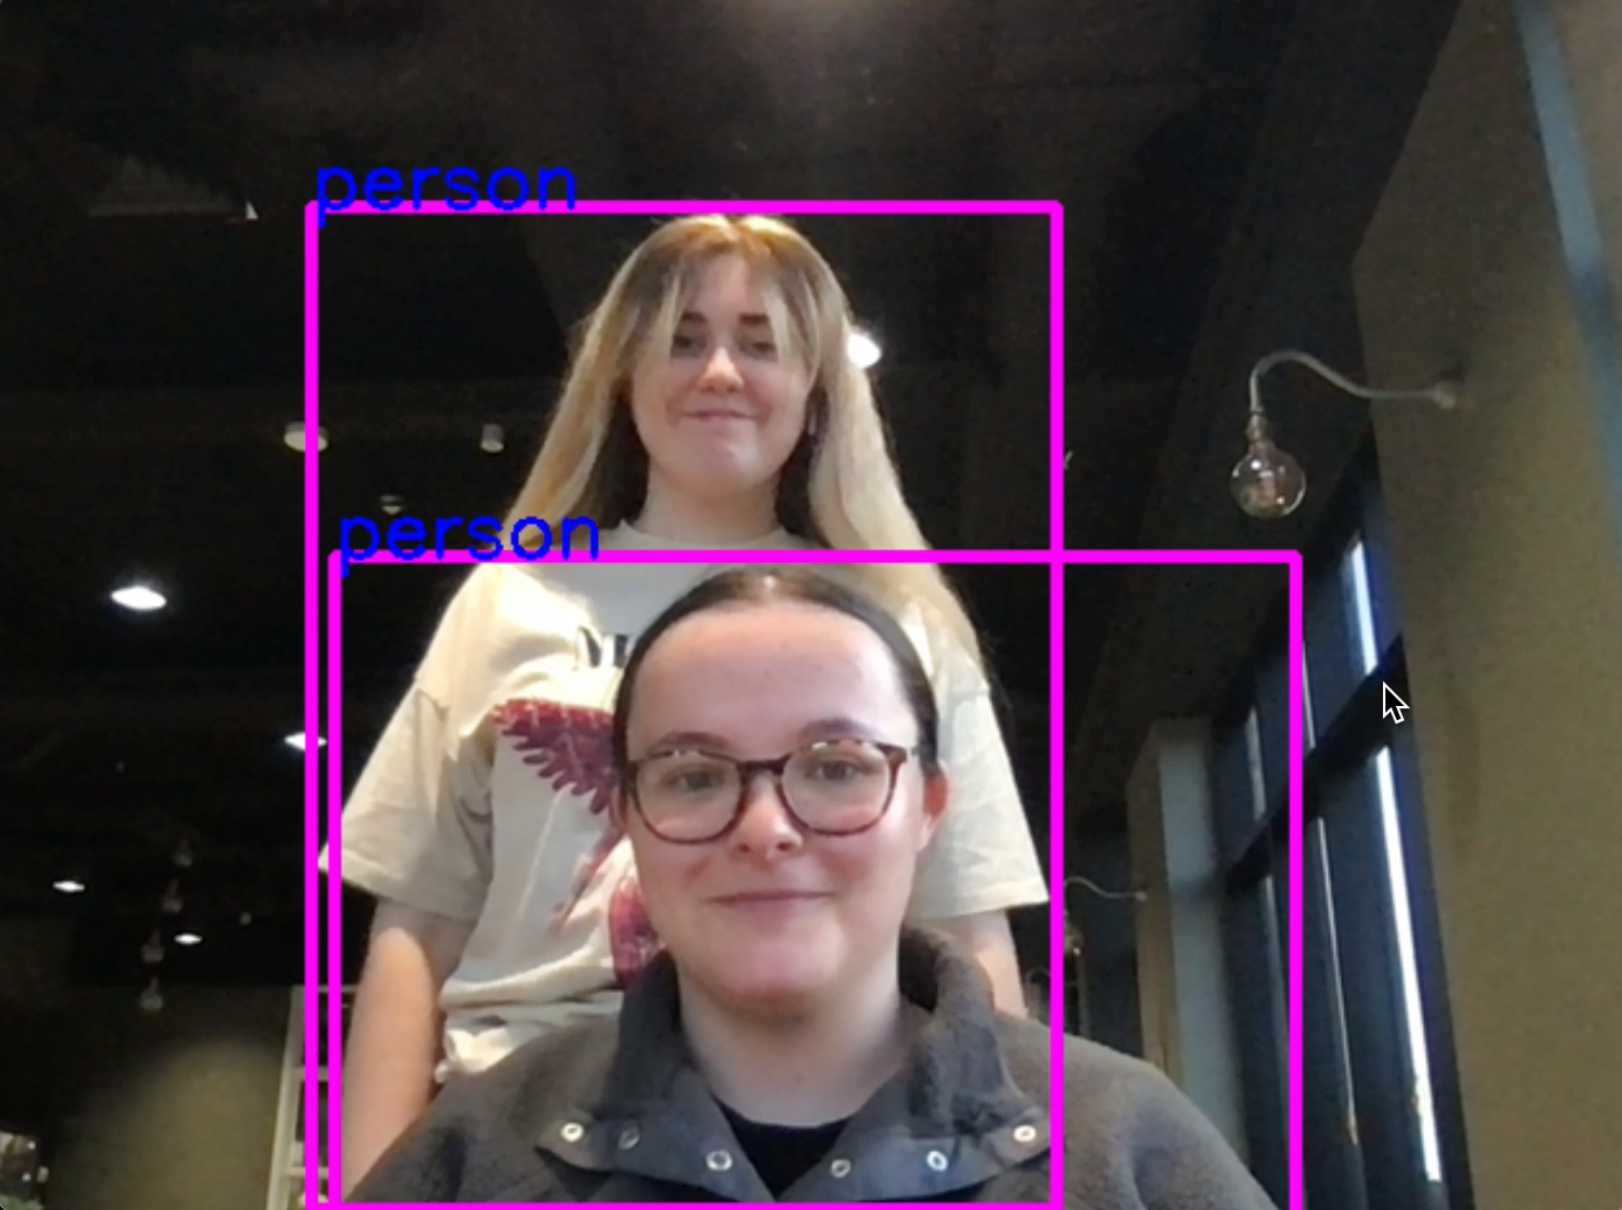
\includegraphics[width=\textwidth]{img/fig1-img1.png}
         \caption{Forward facing}
         \label{fig:a}
     \end{subfigure}
     \hfill
     \begin{subfigure}[b]{0.3\textwidth}
         \centering
         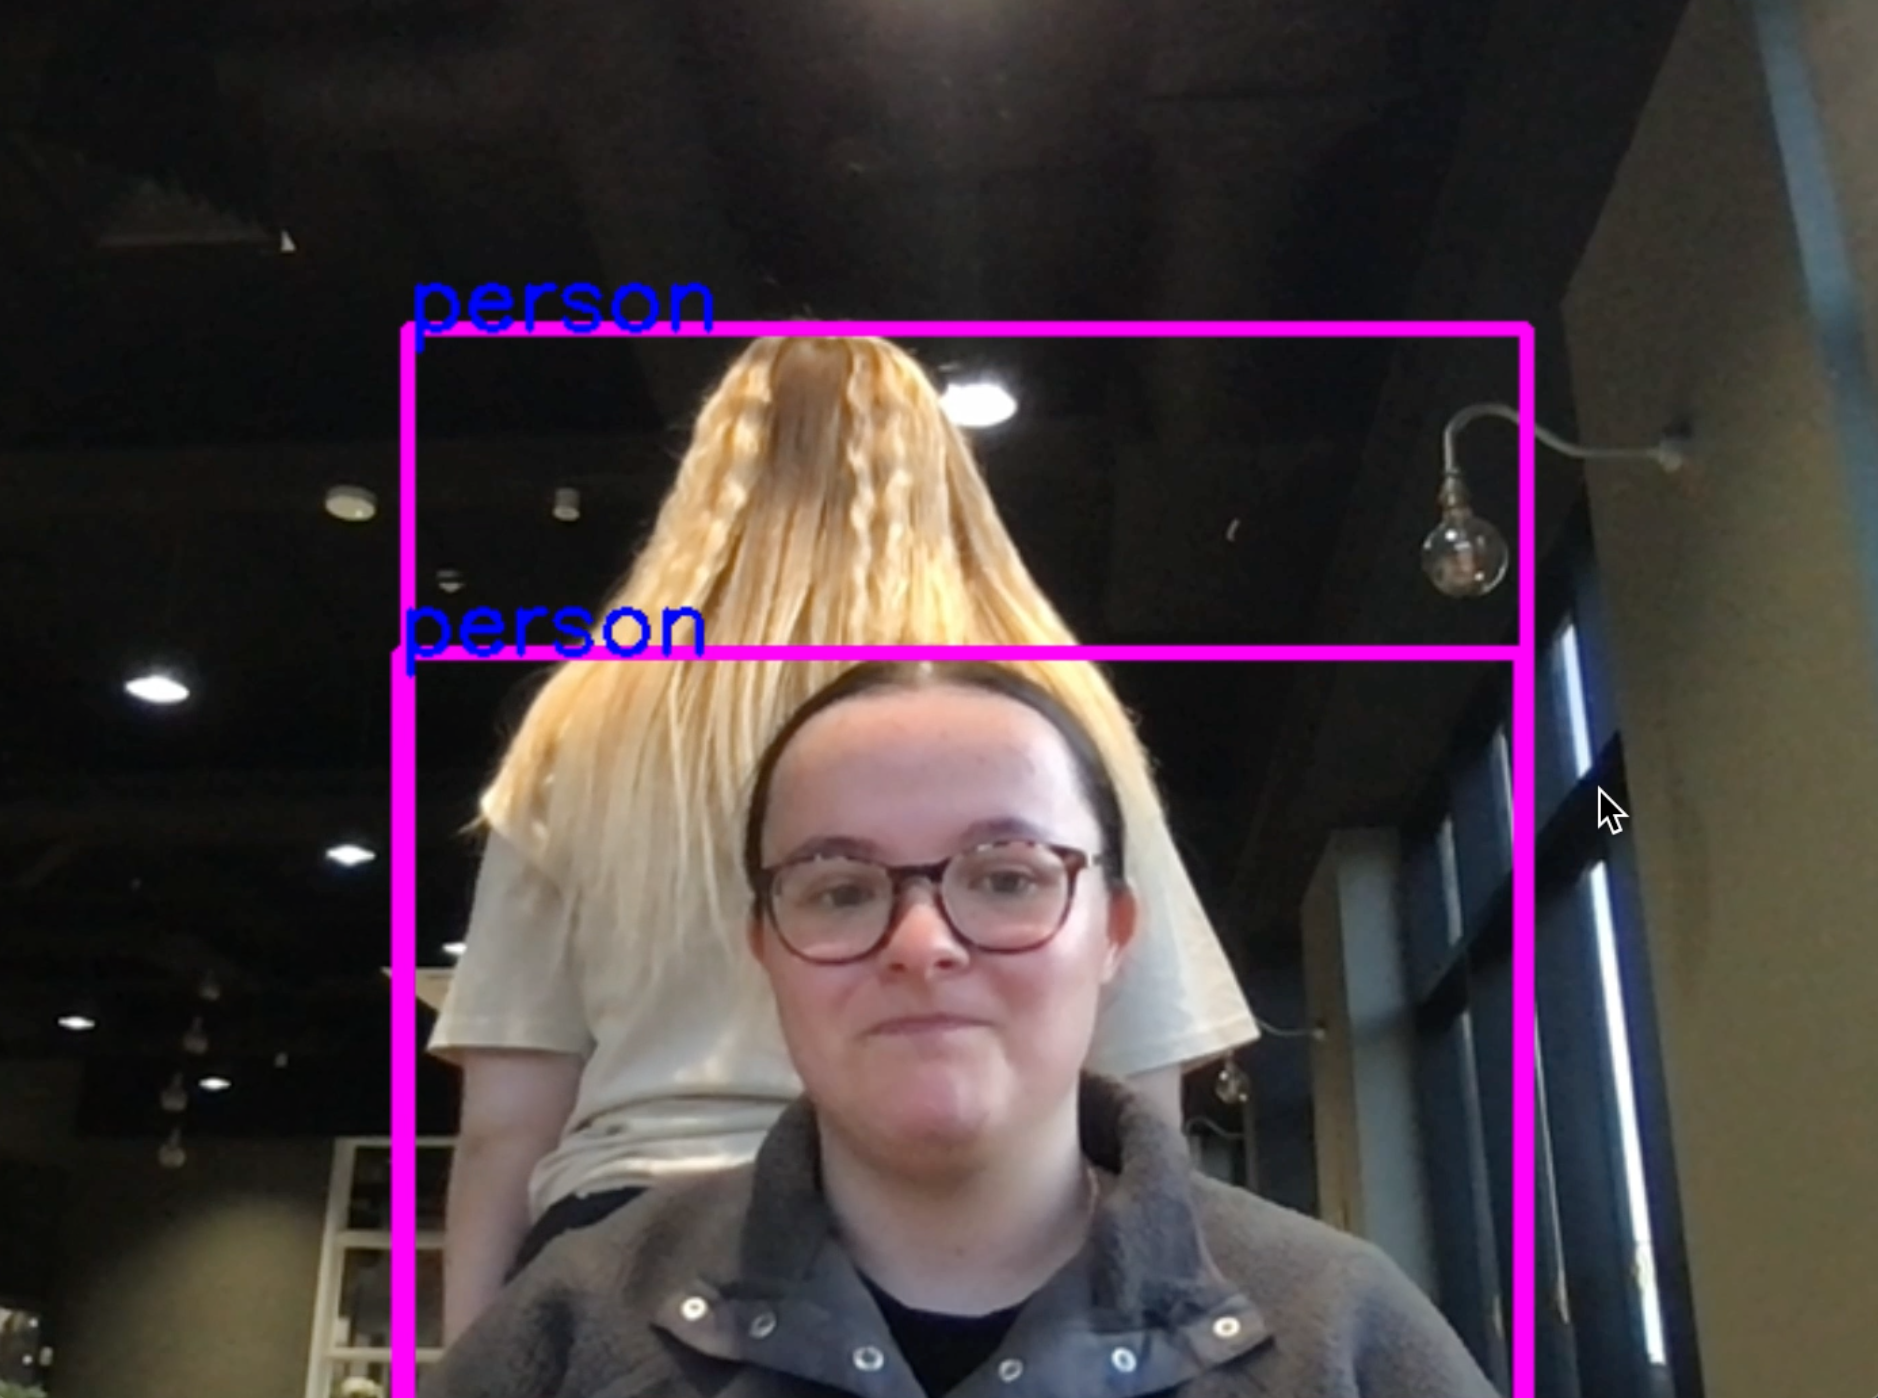
\includegraphics[width=\textwidth]{img/fig1-img2.png}
         \caption{Backward facing}
         \label{fig:b}
     \end{subfigure}
     \hfill
     \begin{subfigure}[b]{0.3\textwidth}
         \centering
         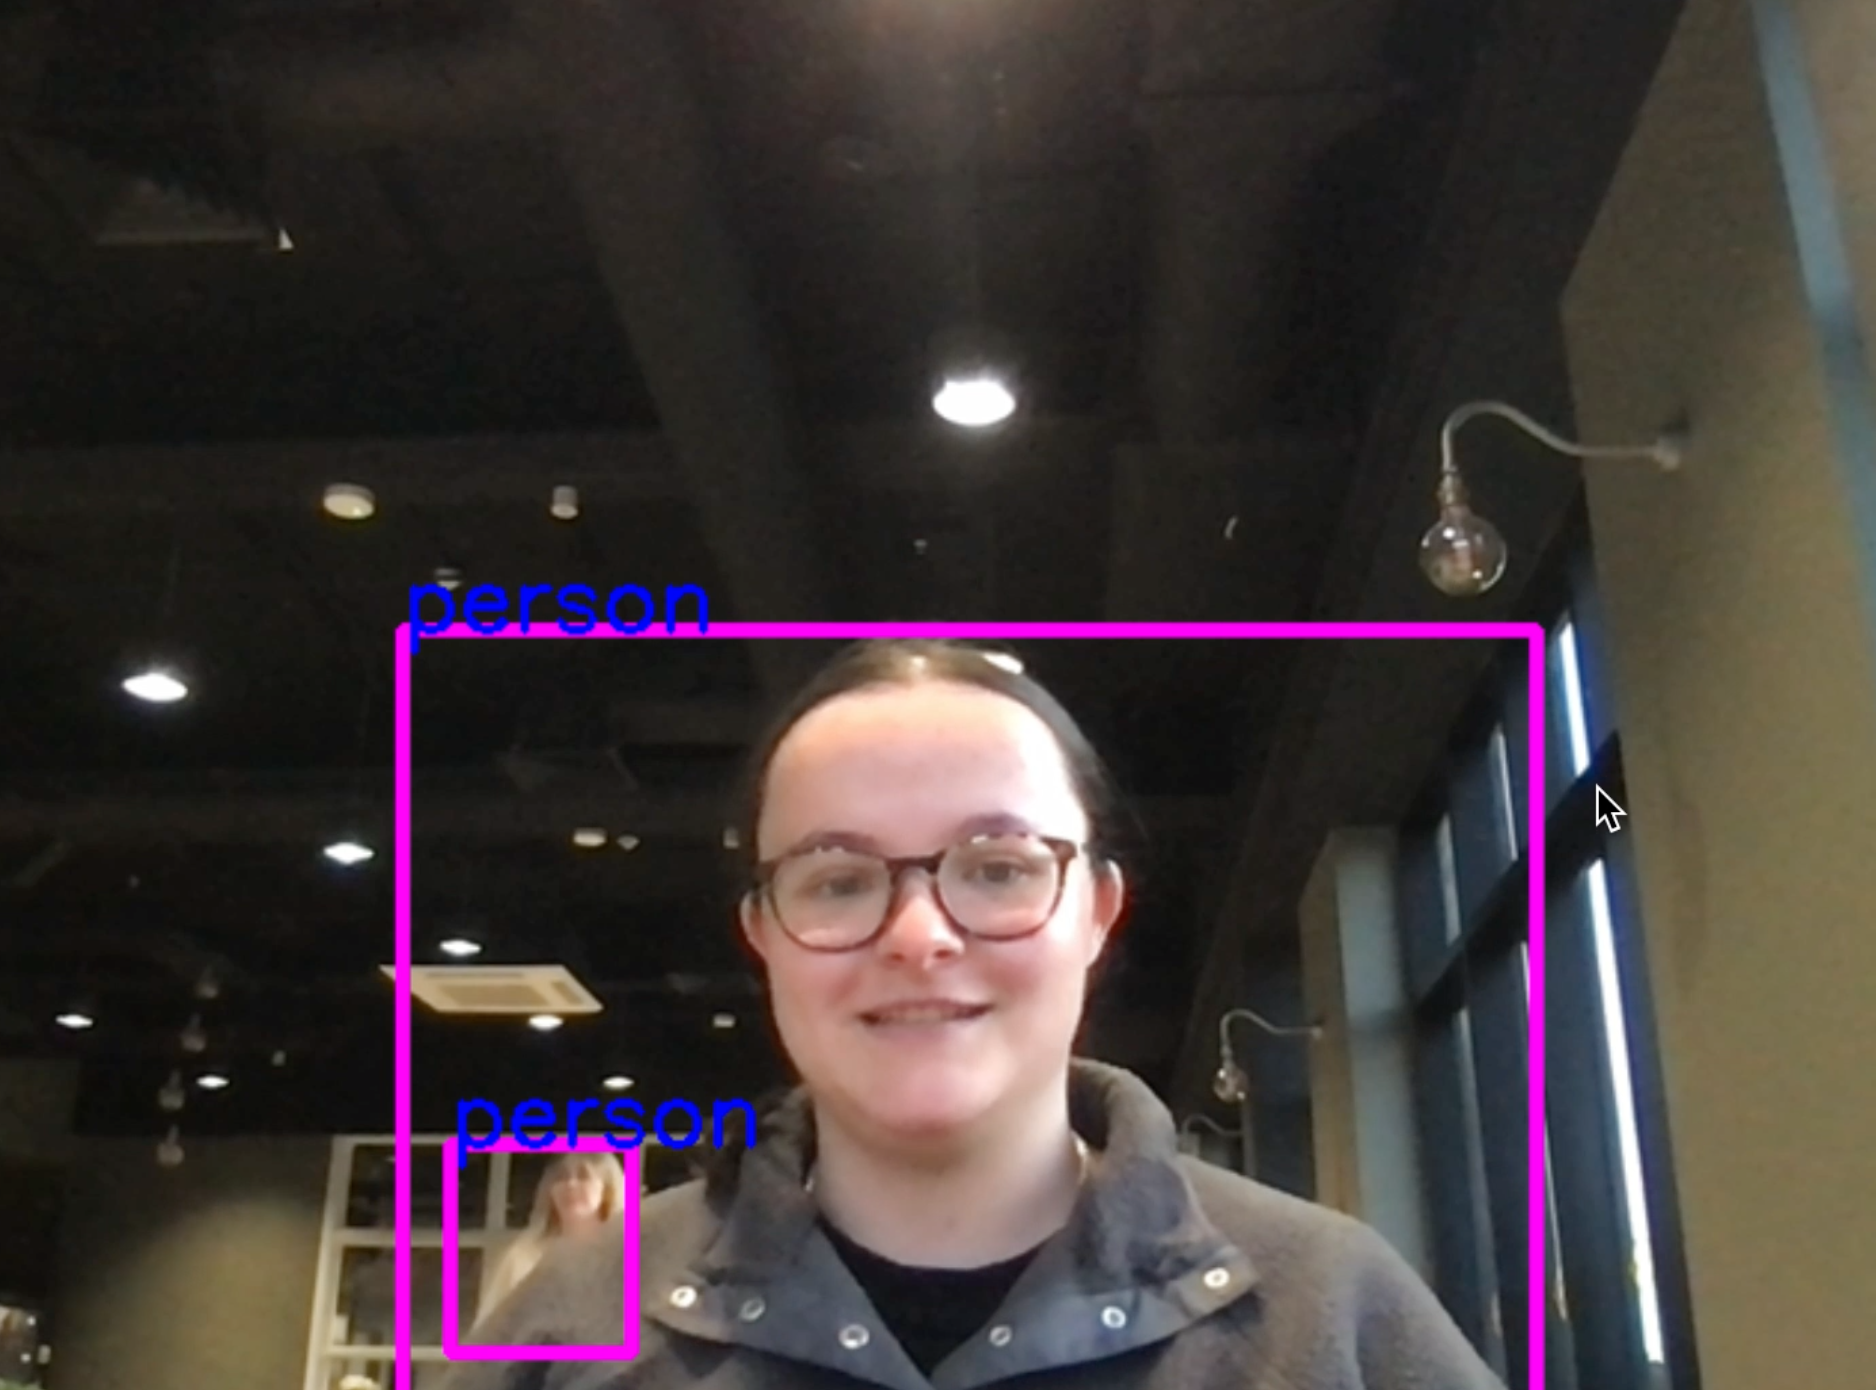
\includegraphics[width=\textwidth]{img/fig1-img3.png}
         \caption{From a distance}
         \label{fig:c}
     \end{subfigure}
        \caption{YOLO being used to detect more than one person in-front of the camera. The observer stands at different distances and angles to test the system.}
        \label{fig:yolo}
\end{figure}

\subsubsection{Eye detection using dlib}
To enable gaze-based detection, dlib was identified as an appropriate solution for its efficient face detection and facial landmark prediction capabilities. Dlib is an open-source software library (King, 2019) including 68-point facial landmark detection model (see figure \ref{fig:facial-landmarks}) that is based on the Histogram of Oriented Gradients (HOG) combined with a linear support vector machine (SVM) which allows for effective detection of faces within the camera (Kazemi & Sullivan, 2014).

The shape predictor in dlib uses multiple regression trees to detect facial landmarks including the eyes, nose and mouth. The model was identified as useful for this project due the accurate feature recognition of multiple people at once allowing for gaze estimations to be calculated.

Before implementation, the model was imported into Python and used to identify any faces with the camera. Figure~\ref{fig:dlib} shows the code being run on an Apple Macbook (720p FaceTime HD camera) to demonstrate how more than one person can be identify when facing forward.

Image \ref{fig:face_a} shows how more than one face can be identified at once where all 68 points are drawn onto the user. Images \ref{fig:face_b} and \ref{fig:face_c} demonstrate how a user cannot be identified when turned around or from approximately 3 meters behind. This highlights that the onlooker would need to present their facial features closely to the camera in order to be identified. Despite these challenged, dlib was identified as computationally efficient and reliable making it a practical choice for gaze detection.


\begin{figure}[h!]
\centering
\fbox{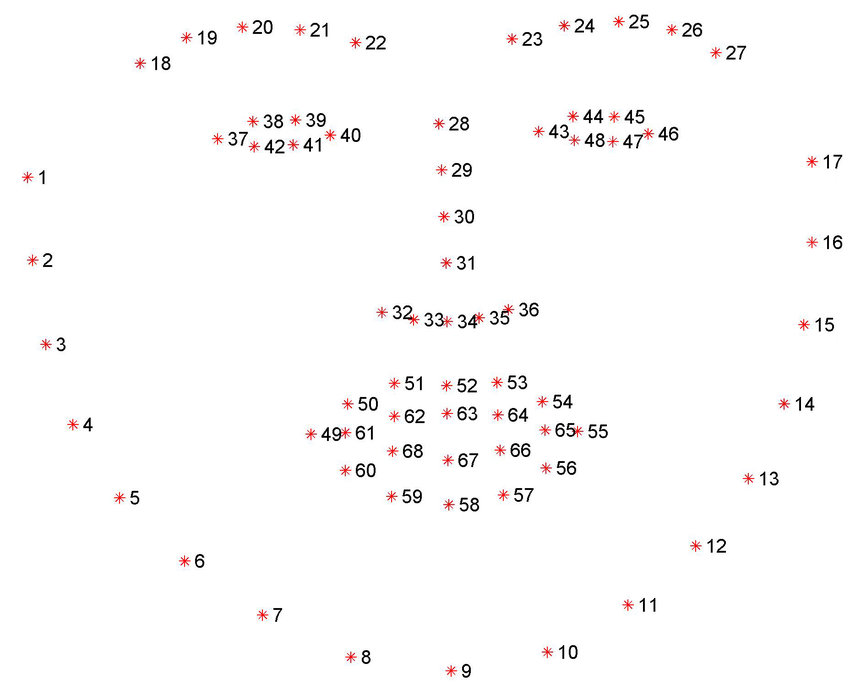
\includegraphics[width=.3\textwidth]{img/facial-landmarks.png}\hfill}

\caption{68 facial landmarks model as part of the dlib library \cite{noauthor_dlib_nodate}. }
\label{fig:facial-landmarks}
\end{figure}

\begin{figure}[h!]
     \centering
     \begin{subfigure}[b]{0.3\textwidth}
         \centering
         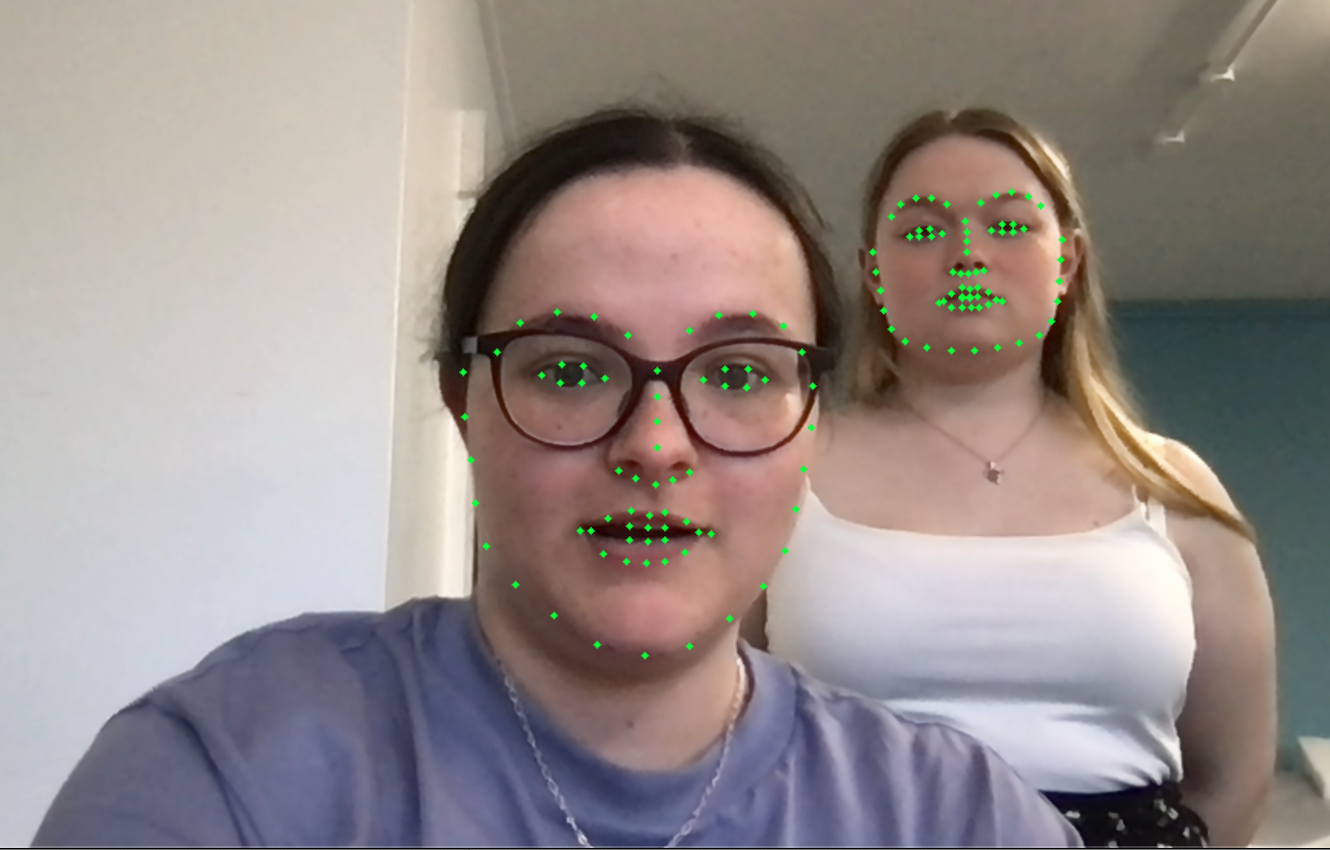
\includegraphics[width=\textwidth]{img/face_img1.png}
         \caption{Forward facing}
         \label{fig:face_a}
     \end{subfigure}
     \hfill
     \begin{subfigure}[b]{0.3\textwidth}
         \centering
         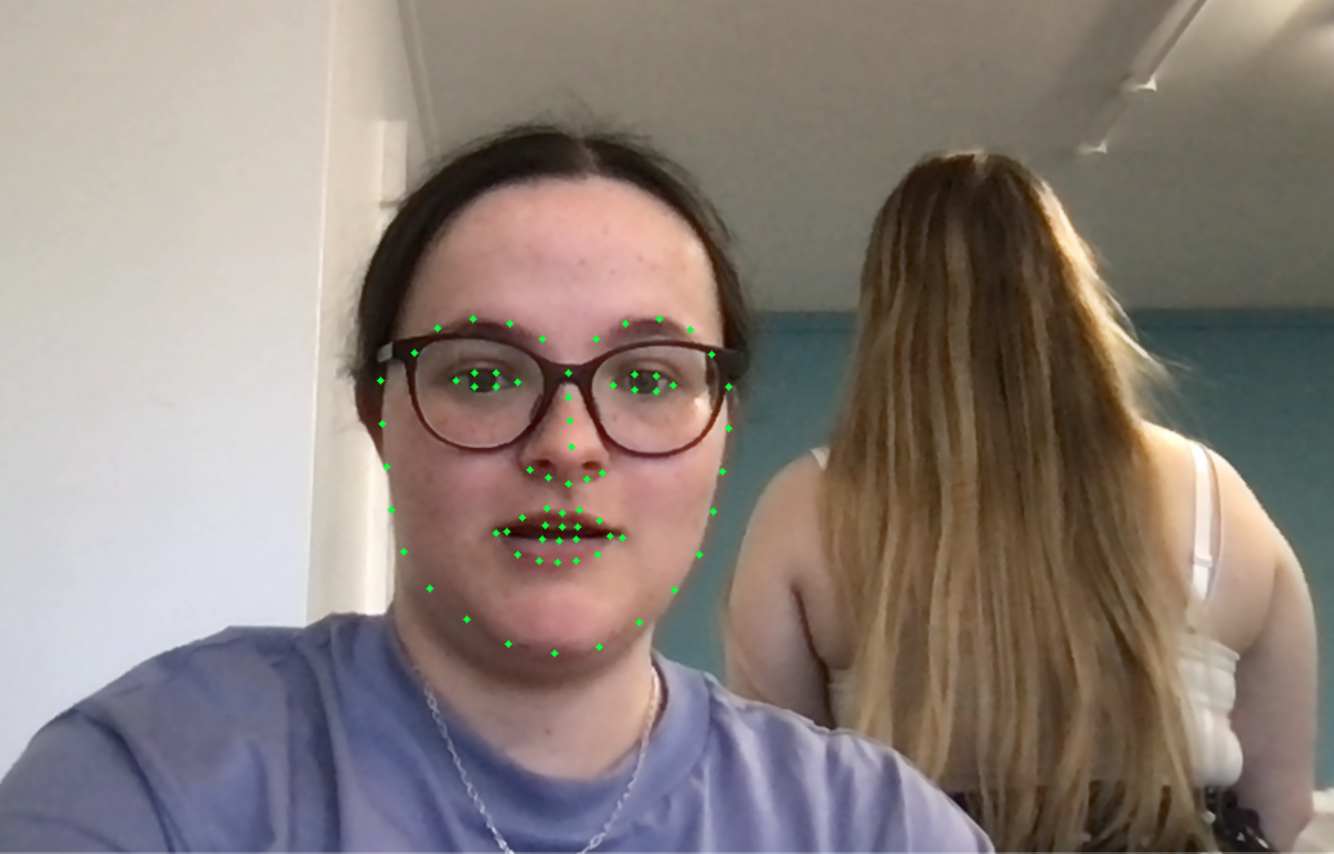
\includegraphics[width=\textwidth]{img/face_img2.png}
         \caption{Backward facing}
         \label{fig:face_b}
     \end{subfigure}
     \hfill
     \begin{subfigure}[b]{0.3\textwidth}
         \centering
         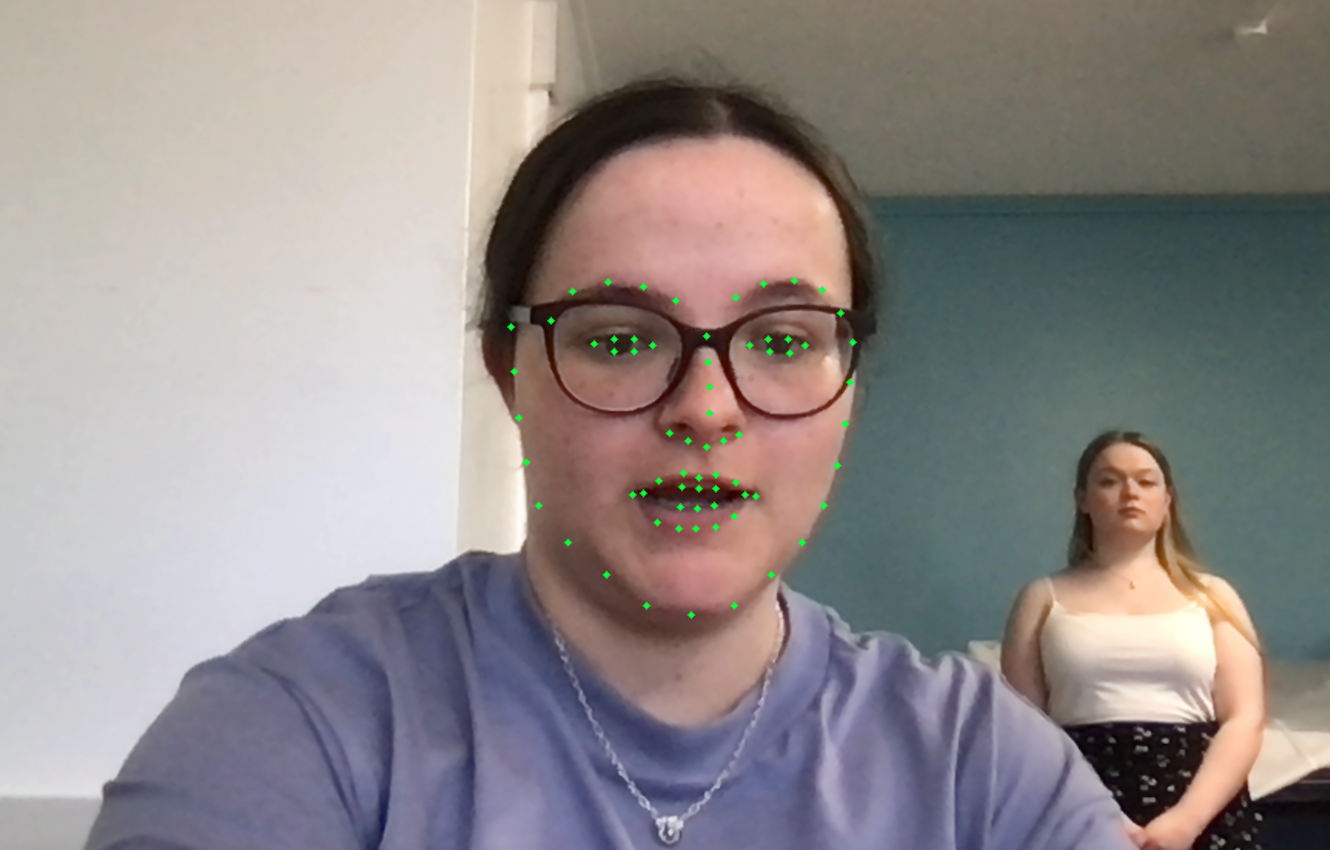
\includegraphics[width=\textwidth]{img/face_img3.png}
         \caption{From a distance}
         \label{fig:face_c}
     \end{subfigure}
        \caption{dlib facial recognition being used to detect more than one person in-front of the camera. The observer stands at different distances and angles to test the system.}
        \label{fig:dlib}
\end{figure}

Together, these models formed the core detection strategies used during prototyping and producing the system. Whilst YOLO was used during the first iteration to broadly identify the presence of more than one person, the dlib library was used during the final solution to accurately identify and track the gaze direction of a potential shoulder surfer. The direct use of these will be discussed during the implementation part of this paper.

\section{Implementation}
\subsection{Overview}

The implementation of the shoulder surfing detection system was produced using a user-centred, iterative development process. The system was built using Python due to its accessibility and wide library support \textcolor{red}{ref here}. The main libraries used include OpenCV \textcolor{red}{ref here} for real-time webcam capture, dlib \textcolor{red}{ref here} for face and landmark detection, and customtkinter \textcolor{red}{ref here} for building the graphical user interface. Testing and development were conducted on a Macbook with a 720p FaceTime HD webcam, although the software was designed to operate cross-platform where possible.
The development was structured into two major phases where the initial prototype relied solely on persona detection using YOLO, while the final version incorporated gaze estimation using dlib’s facial landmark detection. This section describes each phase, the system’s interface and the decisions made to support modularity and responsiveness.

\subsection{Prototype 1: YOLO-Based Detection}

The first version featured a basic graphical interface, consisting only of a start and stop controls hardcoded into the script. These were no adjustable settings or real-time feedback provided to the user. While this minimal interface was sufficient for functional testing, it lacked the usability features required for regular, user-friendly operation.

In this version, the YOLOv8 model for person detection was used due to its ability to detect multiple people at high speed (up to 45 FPS) making is a strong algorithm to help identify the presence of potential shoulder surfers in real time. The model was integrated into the system through the Ultralytics Python interface \textcolor{red}{ref here} and connected to the webcam feed via OpenCV.

The initial logic flagged a potential threat if more than one person was detected within the frame. If this condition was met, the system dimmed the screen and played an audio warning using the playsound library. It was clear from user studies (see \ref{sec:Evaluation}) that while the prototype was effective in detecting people at varying distances and angles, it lacked the ability to recognise whether the user was actually being observe causing false positives especially in busier environments.

\subsection{Prototype 2: Gaze Detection with dlib}

In response to the limitations to the first prototype, the second iteration introduced gaze tracking using dlib’s 68-point facial landmark model. This logic provided a lightweight and efficient method for frontal face detection where once a face was detected, specific landmarks around the eyes were used to estimate gaze direction.

Gaze was approximated by comparing the horizontal and vertical alignment of the pupil relative to the eye corners (see 4.3.1). A custom function determined whether the gaze was focused toward the centre, left or right which allowed the system to infer whether the user was likely looking at the screen. A shoulder surfing threat was only triggered when more than one face was present and the user’s gaze was focused on the screen, significantly reducing false positives from before.

This prototype also introduced a frame counter and delay which means that if a previously detected threat disappeared for a set number of frames, the system automatically restored brightness, improving responsiveness without introducing any major visual changes.

Alongside the improved detection logic, this iteration also introduced a new user interface to address the usability limitation of prototype 1. The updated GUI, discussed in the next section, provided real-time control, visual feedback and configuration options, making the system more user-friendly and practical for everyday use.

\subsubsection{Gaze Calculations}

To estimate gaze direction, the system computes midpoints and defines horizontal and vertical eye reference lines using facial landmarks from dlib's 68-point model. For the right eye:

\begin{itemize}

    \item Let \( P_{43} = (x_{43}, y_{43}) \) and \( P_{46} = (x_{46}, y_{46}) \) denote the outer and inner corners of the right eye.

    \item Let \( P_{44}, P_{45}, P_{48}, P_{47} \) denote the upper and lower eyelid landmarks.

\end{itemize}
The horizontal reference line is defined as:
\[
\text{Horizontal Line}_{\text{right}} = \overline{P_{43}P_{46}}
\]

The vertical reference line uses the midpoint of the upper and lower eyelids:
\[
M_{\text{top}} = \left( \frac{x_{44} + x_{45}}{2}, \frac{y_{44} + y_{45}}{2} \right)
\]

\[
M_{\text{bottom}} = \left( \frac{x_{48} + x_{47}}{2}, \frac{y_{48} + y_{47}}{2} \right)
\]

\[
\text{Vertical Line}_{\text{right}} = \overline{M_{\text{top}}M_{\text{bottom}}}
\]

This calculation is mirrored for the left eye using landmarks \( P_{37} \) through \( P_{42} \). A visual graphic is shown in figure \ref{fig:eye_calc} to help understand where the points are located in real life. In the system, these lines are visualised on the video frame to assist with approximate gaze direction detection. A code snippet of these calculations put into practice are provided in appendix \ref{app:gaze_calcs}.


\begin{figure}[h!]
    \centering
    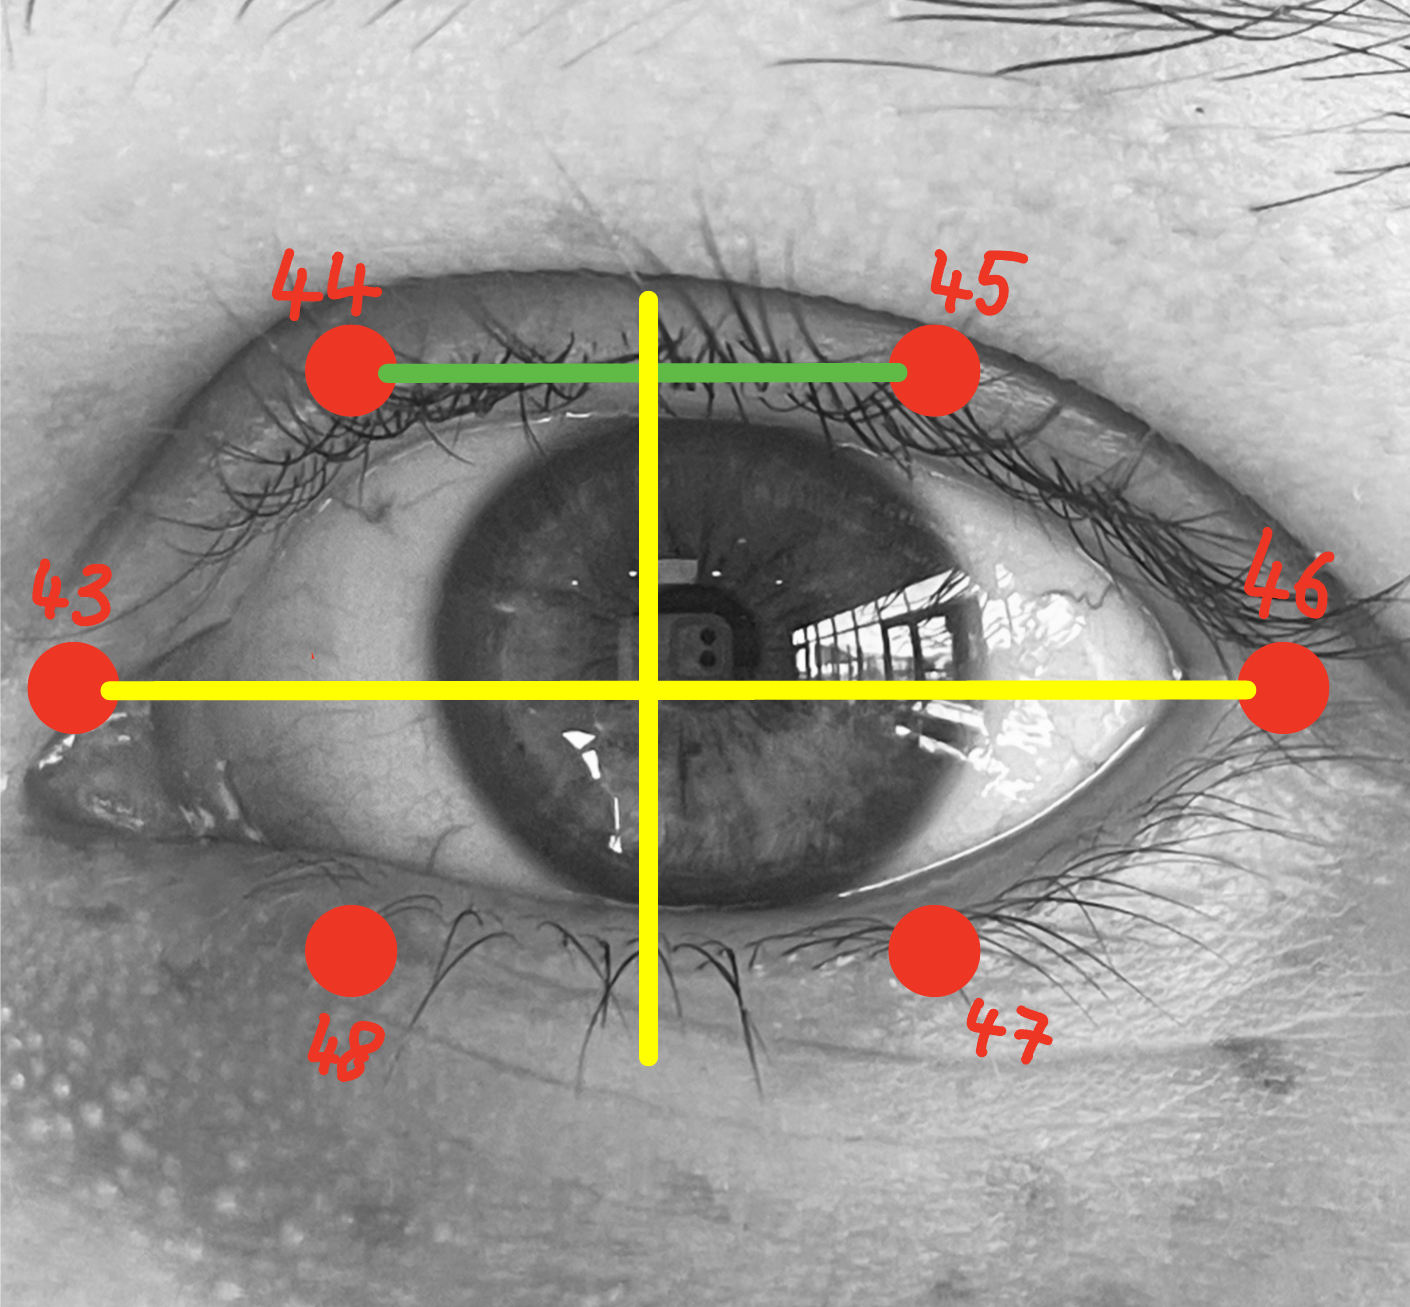
\includegraphics[width=0.6\linewidth]{img/Eye_calc.jpg}
    \caption{Graphic to show key eye point landmark calculations taken from the 68-point landmarks used to detect and track gaze direction in the system.}
    \label{fig:eye_calc}
\end{figure}

\subsection{Graphical User Interface (GUI)}

The GUI (see figure \ref{fig:gui_overview}) was developed using the customtkinter library to offer a modern interface to the user. The sidebar layout was designed to give users easy access to core functions: starting and stopping detection, viewing logs, adjusting dimming brightness and toggling audio alerts.

Controls include:
\begin{itemize}
  \item Start/Stop buttons: Controls the detection, buttons change colour when active.
  \item Brightness slider: Adjusts screen dimming level.
  \item Sound toggle: Enables or disables warning sounds.
  \item Log panel: Displays recent events for transparency and trust.
\end{itemize}

The layout adheres to Don Norman’s usability principles by providing clear feedback, discoverability, and user control. Default settings were chosen for general usability but are customisable for different environments.

\begin{figure}[h!]
  \centering
  \begin{subfigure}[b]{0.45\textwidth}
    \centering
    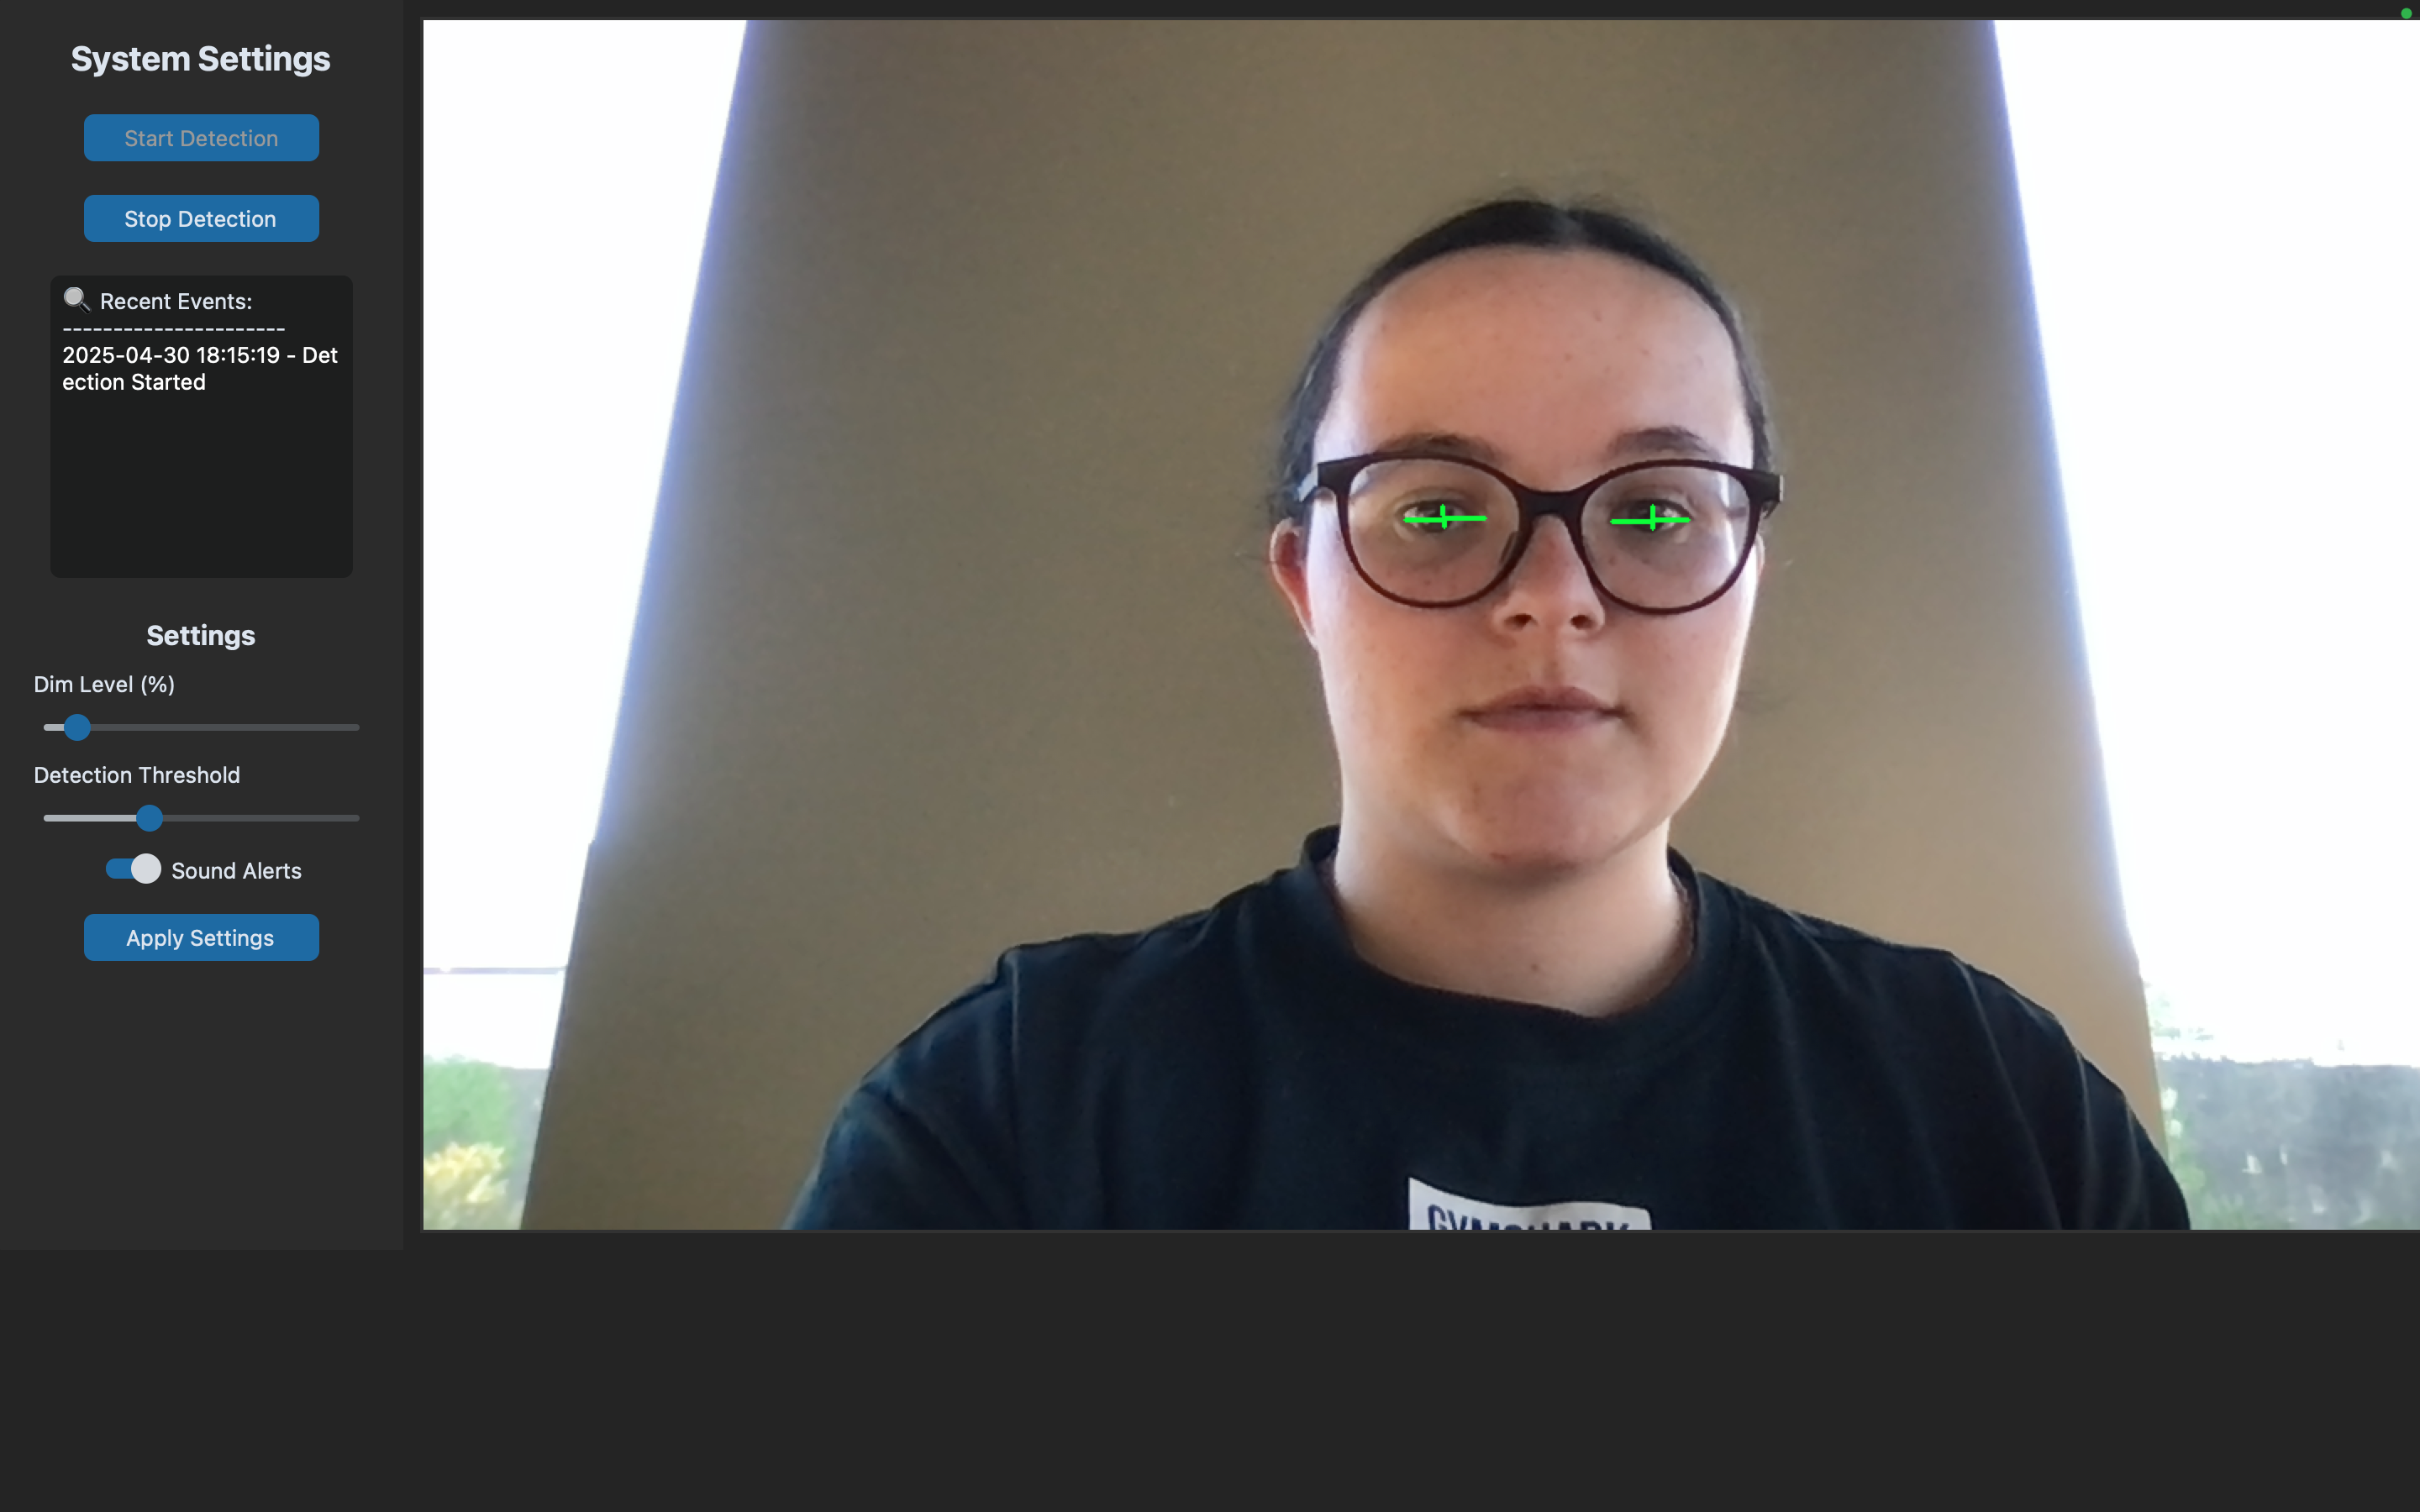
\includegraphics[width=\linewidth]{img/gui.png}
    \caption{System interface with live feed}
    \label{fig:gui_face}
  \end{subfigure}
  \hfill
  \begin{subfigure}[c]{0.45\textwidth}
    \centering
    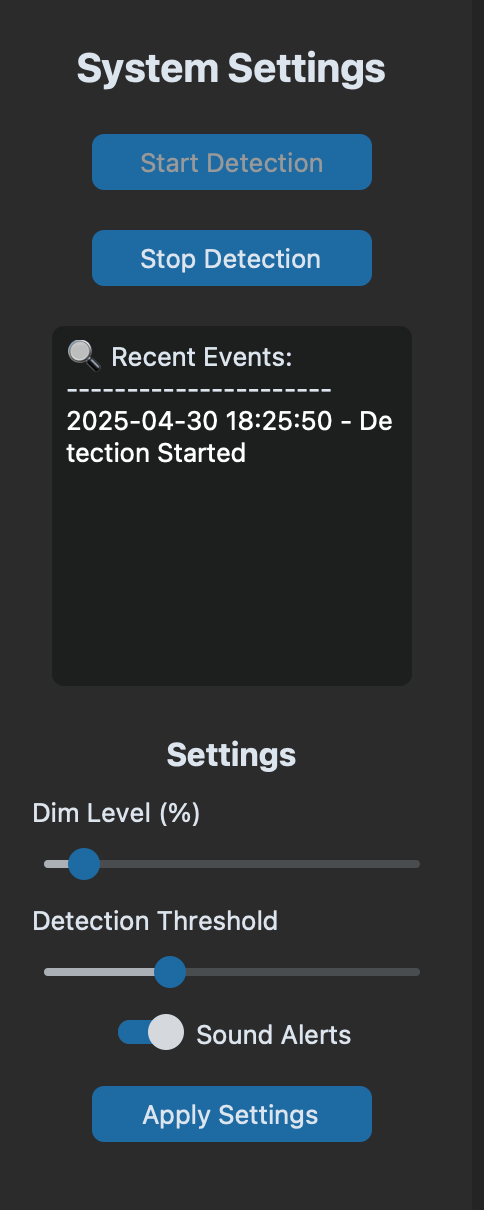
\includegraphics[width=0.6\linewidth]{img/sidebar.png}
    \caption{System control panel}
    \label{fig:gui_controls}
  \end{subfigure}
  \caption{Interface elements showing (a) the detection system in use, and (b) the customisable control panel.}
  \label{fig:gui_overview}
\end{figure}

\subsection{Technical Challenges and Solutions}

Several challenges arose during development:
\begin{itemize}
  \item Brightness control across platforms: On macOS, Python’s screen\textunderscore brightness\textunderscore control library had limited compatibility, so fallback shell commands were used.
  \item False positives in early testing: Without gaze logic, many non-threats triggered alerts. The second prototype addressed this by coupling gaze and presence detection.
  \item Low-light performance: Face and eye detection reduced in dim lighting. Histogram equalisation and threshold tuning were explored to enhance reliability.
  \item Real-time performance: To reduce lag for prototype 1, only every fifth video frame was processed during detection. This reduced CPU load while maintaining responsiveness.
\end{itemize}

These technical improvements ensured the system remained responsive, lightweight, and practical for everyday use. The implementation phase demonstrated the feasibility of real-time, ambient shoulder surfing detection using accessible, open-source tools.

\section{Evaluation}

\subsection{Study Objectives}

To assess the effectiveness and usability of the shoulder surfing detector, a user study was conducted. The aim was to evaluate both the algorithm used to detect people and the user experience when in different scenarios. The study focused on identifying false positives, false negatives, and overall detection accuracy, while also undersntanding the participants perceptions of usability and effectiveness.

Two user studies were carried out where the first involved testing the initial prototype, which relied only on YOLO-based person detection and the second focused on the refined system that used gaze tracking via dlib. The results from the first user study were then used to improve the system and design which resulted in the second study being carried out.

A total of 20 participants took part in the study all with a range of technical experience levels and all followed the below structure:

\begin{itemize}
    \item Pre-task briefing and consent
    \item Observation of system performance during tasks
    \item Post-task questionnaire evaluating usability, perceived effectiveness, and overall trust
\end{itemize}

\subsection{Quantitative Results}

\textbf{Detection Accuracy}

Prototype 1, which used YOLO-based person detection, correctly identified the presence of multiple people but triggered frequent false positives. In contrast, Prototype 2, which used gaze tracking with face detection, significantly reduced false alerts while maintaining threat recognition.
From system logs and manual observation:
\begin{itemize}
    \item Prototype 1: High detection rate but up to 40\% false positives
    \item Prototype 2: Fewer false positives, improved confidence in alerts, and better contextual accuracy (when user gaze confirmed screen focus)
\end{itemize}

After both user studies were conducted, statistical analysis was carried out using Likert-scale responses from the post-study questionnaire. Independent t-tests were used to compare the average scores across four metrics: ease of user, perceived effectiveness, perceived security and interference with normal use.

The results showed a significant improvement in ease of use (p = 0.0051), showing that users found prototype 2 more intuitive that the first version. The most significant change was in interference with normal use (p < 0.0001), where users reported less disruptions in prototype 2 due to the more precise detection algorithm and live feedback. While perceived effectiveness also improved, the difference was not as significant (p = 0.0862), and perceived security remained high across both prototypes (p = 0.4800). To help visualise these results, a plot was created to show the distribution of ease of user ratings for both prototypes where the vertical lines represent the mean scores (see figure \ref{fig:t-test}). These results verified the hypothesis that the gaze tracking within the detection improves user satisfaction and reduces false system alerts.

\begin{figure}
    \centering
    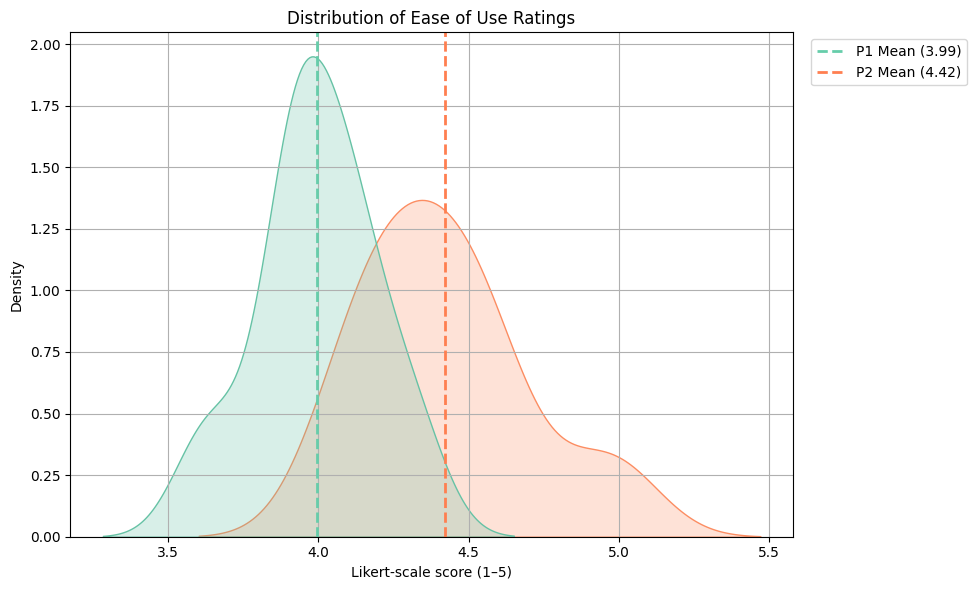
\includegraphics[width=1.0\linewidth]{img/ttest.png}
    \caption{Graph the show the distribution of ease of user ratings from the user studies of both prototypes.}
    \label{fig:t-test}
\end{figure}

\textbf{Usability Scores (Post-Study Questionnaire Highlights)}

Participants rated their experience across several metrics:
\begin{table}[h!]
\centering
\begin{tabular}{|l|c|}
\hline
\textbf{Metric} & \textbf{Avg. Score (out of 5)} \\
\hline
Ease of use & 4.2 \\
Perceived effectiveness & 4.4 \\
Perceived security & 4.3 \\
Interference with normal use & Low (most said “No”) \\
\hline
\end{tabular}
\caption{Participant usability scores from the post-study questionnaire.}
\label{tab:usability_scores}
\end{table}

Participants with prior experience of shoulder surfing rated the system’s usefulness slightly higher. Some noted that while occasional false alerts were acceptable, performance in dim lighting still posed a challenge.

\subsection{Qualitative Results}

Open-ended responses revealed several key themes. Many users appreciated the ambient feedback system, such as the automatic screen dimming and audio alerts, describing these as non-intrusive and effective ways to gain attention without disrupting workflow. The system’s log panel also received positive feedback, with users commenting that it improved transparency and helped them understand why alerts had been triggered.

However, not all feedback was positive. Some participants found that the system struggled in low-light conditions, where detection accuracy dropped noticeably. This limitation led to suggestions for future enhancements, such as incorporating infrared detection or adaptive brightness controls. In earlier iterations of the prototype, several users also expressed frustration with false alerts, though most acknowledged that these issues were largely resolved in the final version.

Participant commentary reflected a range of experiences. One participant mentioned that the system would be particularly useful in shared workspaces where privacy concerns are heightened. Another noted that the system’s reliability improved their sense of security while working in public. These insights support the direction of the design improvements made between prototypes and highlight areas for further refinement.

Example participant comments:

“Helpful for work, especially in shared offices.”

“Would be better if it handled dark rooms more reliably.”

“False alerts were annoying in the earlier version.”

\textbf{Alert Feedback Accuracy}

Participants were asked whether the alerts triggered during the tasks were correct. Most participants reported that alerts were appropriate and timely, particularly in Prototype 2. Prototype 1 had a higher rate of false positives due to its reliance solely on presence detection. In contrast, Prototype 2 demonstrated a more refined approach by validating presence with gaze data, significantly reducing the number of incorrect alerts.


\subsection{Summary of findings}

\begin{table}[h]
\centering
\caption{Comparison of Prototype 1 and 2 Based on Key Performance Features}
\begin{tabular}{|l|l|l|}
\hline
\textbf{Feature} & \textbf{Prototype 1 (YOLO)} & \textbf{Prototype 2 (YOLO + Gaze)} \\
\hline
Detection Speed & High & High \\
False Positives & Frequent & Reduced \\
Gaze Awareness & None & Present \\
Usability Rating & Moderate & High \\
User Control / Settings & None & Full GUI \\
\hline
\end{tabular}
\label{tab:prototype_comparison}
\end{table}

Prototype 2 demonstrated a significant improvement in both perceived and actual performance, validating the decision to incorporate gaze tracking. It maintained system responsiveness while reducing false positives and increasing user trust.

\subsection{Eight Golden Rules of Interface Design}

To further assess the project with design principles, the system was evaluated against Shneiderman’s Eight Golden Rules of Interface Design \cite{}. The following table outlines how each principle was considered throughout the system’s development:

\begin{table}[h!]
\centering
\begin{tabularx}{\textwidth}{|l|X|}
\hline
\textbf{Principle} & \textbf{Comments} \\
\hline
Strive for consistency & The system remains consistent by keeping the layout, button placement and colour themes the same throughout. This contributed to good usability scores and positive feedback during user studies. \\
\hline
Enable frequent users to use shortcuts & Although there are no keyboard shortcuts which may have been beneficial on reflection, settings are able to be preserved between sessions to allow users to operate the system more efficiently. \\
\hline
Offer informative feedback & Feedback was clearly communicated through system logs and alerts, allowing users to understand when and why alerts were triggered. \\
\hline
Design dialogue to yield closure & User uncertainty and cognitive load has been reduced by adding visual confirmation like button colour change once pressed and log messages to highlight what’s happening. \\
\hline
Offer simple error handling & While no large errors occurred during testing, users had control to stop detection or adjust sensitivity, offering a straightforward way to correct issues such as false alerts. \\
\hline
Permit easy reversal of actions & Users could immediately reverse detection or notification settings without penalty which allowed flexibility allowed trial-and-error usage without the fear of irreversible actions. \\
\hline
Support internal locus of control & The design gave users with direct control over all system functions, such as starting/stopping detection and adjusting thresholds, which reinforced confidence in the use of the system. \\
\hline
Reduce short-term memory load & The clear labelling of controls, feedback logs, and minimal need for user recall allowed for a fluid experience, especially for novice users who may be unsure. \\
\hline
\end{tabularx}
\caption{Evaluation categorised into the Eight Golden Rules of Interface Design \cite{} }
\end{table}

\subsection{Discussion}

The user study allowed for insights into how the system preformed and the overall success of the project. Both technical aspects and how the user interacted with the system were assessed and compared to the objectives discussed at the start of this paper:

\begin{itemize}
  \item Implementing face detection and gaze tracking techniques suitable for real-time use.
  \item Designing a responsive user interface that allows users to customise detection sensitivity and feedback settings.
  \item Evaluating the system’s accuracy, usability, and effectiveness through controlled user studies.
  \item Iteratively refining the system based on user feedback and performance data.
\end{itemize}

It was decided that whilst the first prototype was able to detect multiple individuals within the camera view, the number false positives was too high meaning the detection was not accurate enough. The second prototype improved this by using eye gaze calculations in order to detect the presence of another person. Usability feedback from the user study also helped improve the interface allowing for a critical evaluation against Norman’s principles of interaction design \cite{} above (see figure \ref{}).

The second prototype also incorporated a more user-friendly GUI to ensure Shneiderman’s “visibility of system status” and “user control” principles \cite{} were considered. For example, feedback was more informative by producing an output log formatted in an appropriate was and optional settings that the user could remain in control of. The user study helped produce this idea and the second user study helped verify that both novice and expert users found the system more intuitive.

Despite these improvements, some limitations were identified such as how the system still struggled in low-light settings meaning its effectiveness was reduced and more false negatives occurred. Additionally, the reliance on eye landmarks made the detection less beneficial when users were angled slightly away or were wearing glasses. It could be suggested that further work into using hardware like infrared or wide-angle cameras would help mitigate these issues caused as the software would be able to detect at a wide range or the position of the user compared to the screen.

Though limitations were identified, the user studies abled us to significantly improve the system and consider areas that had not be thoroughly thought about. The quantitative results clearly highlighted an increase of usability and how the system can be integrated into daily life which was identified as a core objective in the project.

\section{Conclusion}

This research set out to address the problem of shoulder surfing — a subtle but significant privacy threat when using digital devices in public or shared spaces. The proposed system aimed to mitigate this risk using a novel combination of object detection and gaze tracking, wrapped in a user-friendly and minimally intrusive interface.

The development and evaluation of two successive prototypes demonstrated meaningful progress. Prototype 1, built using YOLO-based detection, served as a functional baseline but suffered from high false-positive rates. In contrast, Prototype 2 combined dlib’s facial landmark tracking with contextual gaze estimation, improving both the accuracy of detection and user satisfaction. The introduction of visual and auditory alerts, along with a customisable GUI, further enhanced user control and confidence.

User studies and statistical analysis confirmed that the refined system achieved key goals: it was easier to use, more accurate in identifying genuine threats, and less disruptive to normal activity. These outcomes reflect the strength of the iterative, user-centred design process that informed the project.

Nevertheless, limitations remain. Performance was still affected by environmental lighting, and the use of a standard webcam restricted detection range. With more time or access to hardware like infrared cameras or dedicated eye trackers, further improvements in robustness and precision could be achieved.

In conclusion, the system offers a promising software-based solution to shoulder surfing that respects user autonomy and blends security with usability — contributing to both the technical and HCI-driven understanding of privacy-preserving interfaces.



Prototype 2 demonstrated a significant improvement in both perceived and actual performance, validating the decision to incorporate gaze tracking. It maintained system responsiveness while reducing false positives and increasing user trust.


\newpage
\printbibliography 

\clearpage\appendix

\section{Calculations for gaze tracking}
\label{app:gaze_calcs}

\lstinputlisting[language=Python, caption={Calculations used for gaze tracking in Python.}, firstline=188, lastline=205]{./listings/Stats.py}

\end{document}
